\documentclass[10pt]{article}\usepackage[]{graphicx}\usepackage[]{color}
%% maxwidth is the original width if it is less than linewidth
%% otherwise use linewidth (to make sure the graphics do not exceed the margin)
\makeatletter
\def\maxwidth{ %
  \ifdim\Gin@nat@width>\linewidth
    \linewidth
  \else
    \Gin@nat@width
  \fi
}
\makeatother

\definecolor{fgcolor}{rgb}{0.345, 0.345, 0.345}
\newcommand{\hlnum}[1]{\textcolor[rgb]{0.686,0.059,0.569}{#1}}%
\newcommand{\hlstr}[1]{\textcolor[rgb]{0.192,0.494,0.8}{#1}}%
\newcommand{\hlcom}[1]{\textcolor[rgb]{0.678,0.584,0.686}{\textit{#1}}}%
\newcommand{\hlopt}[1]{\textcolor[rgb]{0,0,0}{#1}}%
\newcommand{\hlstd}[1]{\textcolor[rgb]{0.345,0.345,0.345}{#1}}%
\newcommand{\hlkwa}[1]{\textcolor[rgb]{0.161,0.373,0.58}{\textbf{#1}}}%
\newcommand{\hlkwb}[1]{\textcolor[rgb]{0.69,0.353,0.396}{#1}}%
\newcommand{\hlkwc}[1]{\textcolor[rgb]{0.333,0.667,0.333}{#1}}%
\newcommand{\hlkwd}[1]{\textcolor[rgb]{0.737,0.353,0.396}{\textbf{#1}}}%

\usepackage{framed}
\makeatletter
\newenvironment{kframe}{%
 \def\at@end@of@kframe{}%
 \ifinner\ifhmode%
  \def\at@end@of@kframe{\end{minipage}}%
  \begin{minipage}{\columnwidth}%
 \fi\fi%
 \def\FrameCommand##1{\hskip\@totalleftmargin \hskip-\fboxsep
 \colorbox{shadecolor}{##1}\hskip-\fboxsep
     % There is no \\@totalrightmargin, so:
     \hskip-\linewidth \hskip-\@totalleftmargin \hskip\columnwidth}%
 \MakeFramed {\advance\hsize-\width
   \@totalleftmargin\z@ \linewidth\hsize
   \@setminipage}}%
 {\par\unskip\endMakeFramed%
 \at@end@of@kframe}
\makeatother

\definecolor{shadecolor}{rgb}{.97, .97, .97}
\definecolor{messagecolor}{rgb}{0, 0, 0}
\definecolor{warningcolor}{rgb}{1, 0, 1}
\definecolor{errorcolor}{rgb}{1, 0, 0}
\newenvironment{knitrout}{}{} % an empty environment to be redefined in TeX

\usepackage{alltt}
\setlength{\textheight}{28cm}
\setlength{\textwidth}{16cm}
\setlength{\footskip}{2mm}
\setlength{\oddsidemargin}{0mm}
\setlength{\evensidemargin}{0mm}
\setlength{\topmargin}{0mm}
\setlength{\headsep}{0mm}
\setlength{\parindent}{0mm}

\usepackage[MeX,OT4,plmath]{polski}
\usepackage[cp1250]{inputenc} 
\usepackage[OT4]{fontenc}
\usepackage[polish]{babel}
\selectlanguage{polish}
\let\lll\undefined
\usepackage{amssymb,amsmath,amsfonts}
\usepackage{graphicx}
\IfFileExists{upquote.sty}{\usepackage{upquote}}{}

\begin{document}

\section{Zadanie 8.2}

\begin{knitrout}
\definecolor{shadecolor}{rgb}{0.969, 0.969, 0.969}\color{fgcolor}\begin{kframe}
\begin{alltt}
\hlcom{# 8.2}

\hlstd{m} \hlkwb{<-} \hlkwd{read.table}\hlstd{(}\hlstr{"http://www.ipipan.eu/~teisseyrep/TEACHING/SAR/DANE/Miasta.txt"}\hlstd{,}
    \hlkwc{header} \hlstd{=} \hlnum{TRUE}\hlstd{)}
\hlkwd{head}\hlstd{(m)}
\end{alltt}
\begin{verbatim}
##             Work Price Salary
## Amsterdam   1714  65.6   49.0
## Athens      1792  53.8   30.4
## Bogota      2152  37.9   11.5
## Bombay      2052  30.3    5.3
## Brussels    1708  73.8   50.5
## BuenosAires 1971  56.1   12.5
\end{verbatim}
\begin{alltt}
\hlcom{# a) standaryzacja zmiennych}

\hlstd{mm} \hlkwb{<-} \hlkwd{scale}\hlstd{(m)}

\hlcom{# inny sposob (taki po koleji)}

\hlstd{sr} \hlkwb{<-} \hlkwd{numeric}\hlstd{(}\hlnum{3}\hlstd{)}
\hlstd{sd} \hlkwb{<-} \hlkwd{numeric}\hlstd{(}\hlnum{3}\hlstd{)}

\hlkwa{for} \hlstd{(i} \hlkwa{in} \hlnum{1}\hlopt{:}\hlnum{3}\hlstd{) \{}
    \hlstd{sr[i]} \hlkwb{<-} \hlkwd{mean}\hlstd{(m[, i])}
    \hlstd{sd[i]} \hlkwb{<-} \hlkwd{sd}\hlstd{(m[, i])}
\hlstd{\}}

\hlkwa{for} \hlstd{(i} \hlkwa{in} \hlnum{1}\hlopt{:}\hlnum{3}\hlstd{) \{}
    \hlstd{m[, i]} \hlkwb{<-} \hlstd{(m[, i]} \hlopt{-} \hlstd{sr[i])}\hlopt{/}\hlstd{sd[i]}
\hlstd{\}}

\hlcom{# b) dla Work i Price wyznaczyc kierunki wzdluz ktorych wystepuje najwieksza}
\hlcom{# zmiennosc; wykres rozproszenia}

\hlstd{pc1} \hlkwb{<-} \hlkwd{princomp}\hlstd{(}\hlopt{~}\hlstd{.,} \hlkwc{cor} \hlstd{=} \hlnum{FALSE}\hlstd{,} \hlkwc{data} \hlstd{=} \hlkwd{as.data.frame}\hlstd{(mm[,} \hlnum{1}\hlopt{:}\hlnum{2}\hlstd{]))}

\hlcom{# wybieramy albo macierz korelacji albo kowariancji - mamy zestandaryzowane}
\hlcom{# dane, wiec juz korelacja nie jest potrzebna}

\hlkwd{names}\hlstd{(pc1)}
\end{alltt}
\begin{verbatim}
## [1] "sdev"     "loadings" "center"   "scale"    "n.obs"    "scores"  
## [7] "call"
\end{verbatim}
\begin{alltt}
\hlkwd{head}\hlstd{(pc1}\hlopt{$}\hlstd{scores)}  \hlcom{# Comp.1 to z1, a Comp.2 to z2}
\end{alltt}
\begin{verbatim}
##              Comp.1   Comp.2
## Amsterdam    0.5242  0.82168
## Athens      -0.1823  0.89543
## Bogota      -2.1680 -0.03904
## Bombay      -2.0137  0.61779
## Brussels     0.8196  0.57493
## BuenosAires -0.8323  0.09339
\end{verbatim}
\begin{alltt}
\hlstd{pc1}\hlopt{$}\hlstd{loadings}  \hlcom{# wektory ladunkow (pierwsza kolumna to a1, a druga to a2) -> }
\end{alltt}
\begin{verbatim}
## 
## Loadings:
##       Comp.1 Comp.2
## Work  -0.707 -0.707
## Price  0.707 -0.707
## 
##                Comp.1 Comp.2
## SS loadings       1.0    1.0
## Proportion Var    0.5    0.5
## Cumulative Var    0.5    1.0
\end{verbatim}
\begin{alltt}
\hlkwd{plot}\hlstd{(mm[,} \hlnum{1}\hlstd{], mm[,} \hlnum{2}\hlstd{])}
\hlkwd{abline}\hlstd{(}\hlkwd{c}\hlstd{(}\hlnum{0}\hlstd{,} \hlopt{-}\hlnum{1}\hlstd{),} \hlkwc{col} \hlstd{=} \hlstr{"red"}\hlstd{)}
\hlkwd{abline}\hlstd{(}\hlkwd{c}\hlstd{(}\hlnum{0}\hlstd{,} \hlnum{1}\hlstd{),} \hlkwc{col} \hlstd{=} \hlstr{"blue"}\hlstd{)}
\end{alltt}
\end{kframe}
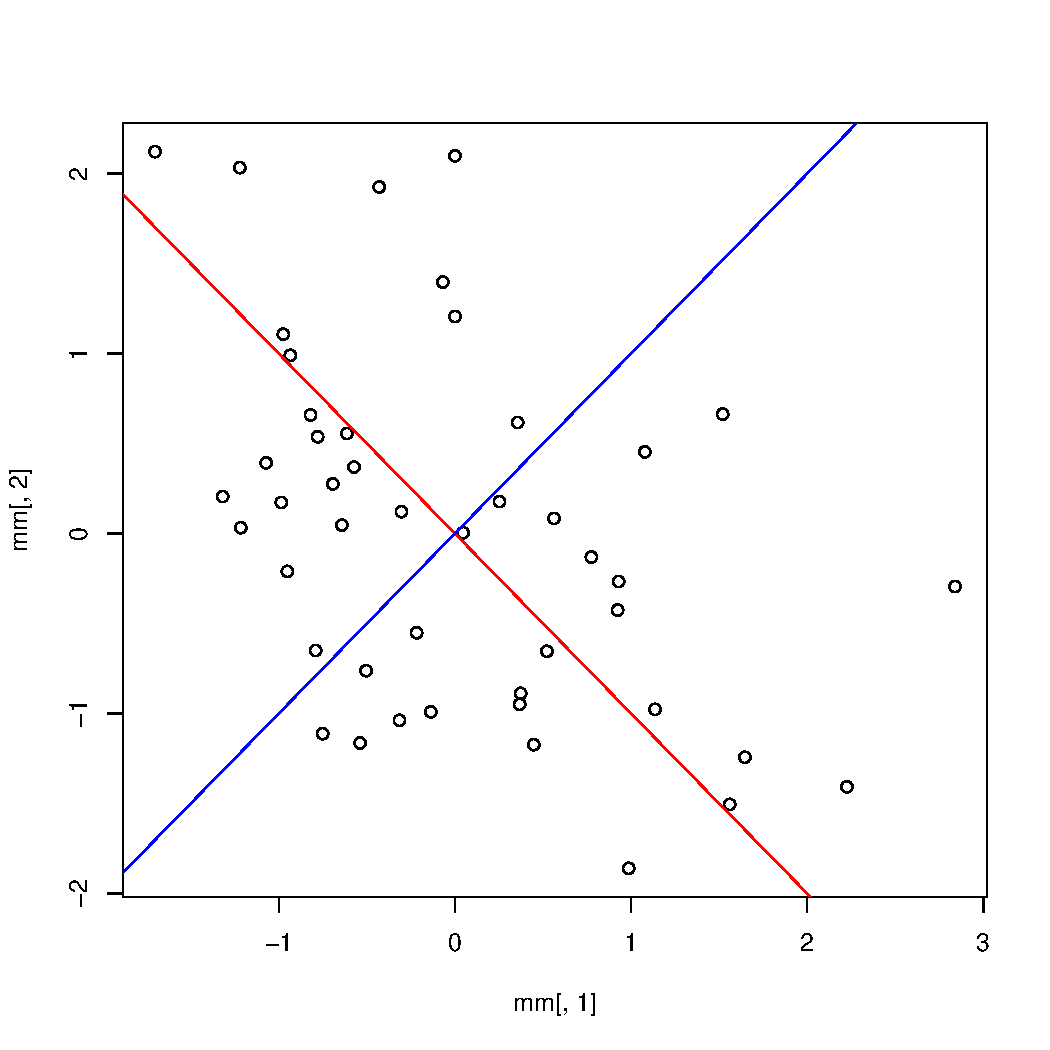
\includegraphics[width=\maxwidth]{figure/unnamed-chunk-1} 

\end{knitrout}


\end{document}











































































